\section{Practical Methodology} 

  \subsection{Model Selection} 

    We've talked about the theory and implementation behind all these models, but in practice, how do we even use them? If we are trying to predict lung cancer in a patient, do we use linear regression, a nonparametric model, or something else? It's not clear at all what to do with the data. Unfortunately, this just comes with domain expertise and experience with data, but we can provide some general pointers. 

    As stated before, we have the flexibility to choose whatever model to train on. So how do we choose which form is the best? Well this is just an assumption that most researchers make, and this is called \textbf{model selection}. 

    \begin{example}[Polynomial Regression]
      The number of terms $M$, i.e. the degree $M-1$ of the polynomial 
        \[h_{\boldsymbol{\theta}} (x) = w_0 + w_1 x + w_2 x^2 + \ldots + w_{M-1} x^{M-1}\]
      in polynomial regression gives us models with different complexities, where $\mathcal{M}_M$ determines the model with a $M-1$th degree polynomial. 
    \end{example}

    \begin{example}
      Suppose I have data sampled data $x^{(1)}, \ldots, x^{(N)}$ on age at death for $N$ people from an unknown distribution $X$. Then, possible models that model the distribution are 

      \begin{enumerate}
        \item $\mathcal{M}_1$: the exponential distribution $p(x \mid \lambda) = \lambda e^{-\lambda y}$ with parameter $\theta = \lambda$. 
        \item $\mathcal{M}_2$: the gamma distribution $p(y \mid a, b) = (b^a / \Gamma(a)) y^{a - 1} e^{- by}$ with parameter $\boldsymbol{\theta} = (a, b)$. 
        \item $\mathcal{M}_3$: the log-normal distribution with $X \sim N (\mu, \sigma^2)$ where ${\boldsymbol{\theta}} = (\mu, \sigma^2)$. 
      \end{enumerate}
    \end{example}

    \begin{example}
      A mixture of Gaussians model 
        \[p(\mathbf{y}) = \sum_{m=1}^M \pi_m N(\mathbf{y} \mid \boldsymbol{\mu}_m, \boldsymbol{\Sigma}_m )\]
      has submodels where we must determine the number of Gaussians $M$. 
    \end{example}

    Now if we assume that the actual true distribution $X$ or the true regressor $\mathbb{E}[Y\mid X]$ is contained within our model $\mathcal{M}$, then we say our model is \textbf{well-specified}. But since researchers have no idea what the data generating process is, so $\mathbb{E}[Y\mid X] \not\in \mathcal{M}$. Hence there is the saying that saying that ``all models are wrong," since we never know what the true data generating process is, and thus the quantity 

      \[\mathbb{E}[Y \mid X] - h_{\boldsymbol{\theta}}^\ast (X)\]

    where $h_{\boldsymbol{\theta}}^\ast (X)$ is the optimized hypothesis functions within $\mathcal{M}$, will always be nonzero. How close we can get this quantity to $0$ determines how useful the model is, and a misspecified model is fundamentally a convenient (or even necessary) assumption on the distribution underlying the data, which may only be a reasonable approximation. 

  \subsection{Feature Engineering} 

    This is also very domain specific. 

  \subsection{Data Preprocessing}

    \subsubsection{Feature Extraction}

      The simplest linear function for regression is simply 
      \[h_\mathbf{w} (\mathbf{x}) = w_0 + w_1 x_1 + \ldots + w_D x_D\]
      This is called linear regression not because $h$ is a linear function of $\mathbf{x}$. It is a linear function of $\mathbf{w}$. Therefore, we can fix nonlinear functions $\phi_j (\mathbf{x})$ and consider linear combinations of them. 

        \[h_\mathbf{w} (\mathbf{x}) = w_0 + \sum_{j=1}^{M-1} w_j \phi_j (\mathbf{x})\]

      We usually choose a dummy basis function $\phi_0 (\mathbf{x}) = 1$ for notational convenience, so that if $\boldsymbol{\phi}$ is the vector of the function $\phi_j$, then we can write $h_\mathbf{w} (\mathbf{x}) = \mathbf{w}^T \boldsymbol{\phi} (\mathbf{x})$. This mapping from the original variables $\mathbf{x} \in \mathbb{R}^D$ to the basis functions $\{\phi_j (\mathbf{x})\}$, which span a linear function space of dimension $M$, is called \textbf{preprocessing} or \textbf{feature extraction} of the data. 

      \begin{example}
        Here are some examples of how we can extract features. 
        \begin{enumerate}
          \item The mapping from a single variable $x$ to its powers 
            \begin{equation}
              x \mapsto (1, x, x^2, \ldots, x^{M-1})
            \end{equation}
          \item The mapping from a configuration of $K$ atoms with their momenta in $\mathbb{R}^{6K}$ to their atomic cluster expansion polynomials. 
          \item The Legendre polynomials, which form an orthonormal basis in the space of polynomials. 
          \item Using equally spaced Gaussian basis functions over the dataset. 
        \end{enumerate}
      \end{example}

      Changing the input space from $D$ dimensions to $M$ dimensions (i.e. extracting our $M$ features) gives the design matrix 
      \begin{equation}
        \mathbf{X} = \begin{pmatrix} 
          \mathbf{x}^{(1)} \\ \mathbf{x}^{(2)} \\ \mathbf{x}^{(3)} \\ \vdots \\ \mathbf{x}^{(n)} \end{pmatrix} \implies \boldsymbol{\Phi} = \begin{pmatrix}
        \text{---} & \phi(\mathbf{x}^{(1)}) & \text{---} \\
        \text{---} & \phi(\mathbf{x}^{(2)}) & \text{---} \\
        \vdots & \vdots & \vdots \\
        \text{---} & \phi(\mathbf{x}^{(n)}) & \text{---}
        \end{pmatrix}
      \end{equation}


      We have shown that the $\texttt{PolynomialFeatures}$ transformer converts our features to a polynomial basis. We can do this for an arbitrary number of features, for example if we map $D = 2$ to a second degree polynomial, we would have the transformation 

      \[(x_1, x_2) \mapsto (1, x_1, x_2, x_1^2, x_1 x_2, x_2^2)\]

      \begin{lstlisting}
      >>> import numpy as np
      >>> from sklearn.preprocessing import PolynomialFeatures
      >>> X = np.arange(6).reshape(3, 2)
      >>> X
      array([[0, 1],
             [2, 3],
             [4, 5]])
      >>> poly = PolynomialFeatures(2)
      >>> poly.fit_transform(X)
      array([[ 1.,  0.,  1.,  0.,  0.,  1.],
             [ 1.,  2.,  3.,  4.,  6.,  9.],
             [ 1.,  4.,  5., 16., 20., 25.]])
      \end{lstlisting}
      Sometimes, we are only worried about the interaction terms among features, so we can set the parameter \texttt{interaction\_only=True}, which would, in the third degree case, transform the features 

        \[(x_1, x_2, x_3) \mapsto (1, x_1, x_2, x_3, x_1 x_2, x_1 x_3, x_2 x_3, x_1 x_2 x_3)\]

      \textbf{Spline transformers} are piecewise polynomials, which is also built in. We notice that it is cumbersome to transform the dataset \texttt{X} with the transformer, store it into another variable, and train the model on that. We can ``combine" the transforming (even multiple layers of transformers) and the model by implementing a ``pipeline," which is initialized by inputting a list of tuples (name and the object) and has the same methods as the model. 

      \begin{lstlisting}
      from sklearn.pipeline import Pipeline
      model = Pipeline([("poly_transform", PolynomialFeatures(degree=2)), 
                        ("lin_regression", LinearRegression())
                        ]) 
      model.fit(X, y)
      \end{lstlisting}

      Now, let's talk about how we can implement a custom transformer. We basically have to create a new subclass that implements the \texttt{fit} (which always returns \texttt{self}) and the \texttt{transform} (which returns the transformed matrix) methods. Here we show for Gaussian basis functions. 

      \begin{lstlisting}
      from sklearn.base import BaseEstimator, TransformerMixin

      class GaussianFeatures(BaseEstimator, TransformerMixin):
          """Uniformly spaced Gaussian features for one-dimensional input"""
          
          def __init__(self, N, width_factor=2.0):
              self.N = N
              self.width_factor = width_factor
              
          def fit(self, X, y=None):
              # create N centers spread along the data range
              self.centers_ = np.linspace(X.min(), X.max(), self.N)
              self.width_ = self.width_factor * (self.centers_[1] - self.centers_[0])
              return self
              
          def transform(self, X): 
              transformed_rows = []
              for mu in self.centers_: 
                  transformed_rows.append(stats.norm.pdf(X, mu, self.width_))
              
              return np.hstack(tuple(transformed_rows))

      model = Pipeline([("gauss_transform", GaussianFeatures(20)), 
                        ("lin_regression", LinearRegression())
                        ]) 

      N = 60
      X = np.random.uniform(-1, 1, size=(N, 1)) 
      Y = true_func(X) + np.random.normal(0, 0.3, size=(N, 1)) 

      model = Pipeline([("gauss_transform", GaussianFeatures(10)), 
                    ("lin_regression", LinearRegression())
                    ]) 
      model.fit(X, Y)
      \end{lstlisting} 

      If we would like to impelment the fourier expansion of a function of form 

        \[f(x) = \frac{1}{2} a_0 + \sum_{n=1}^N a_n \cos(n x) + \sum_{n=1}^N b_n \sin(n x)\]

      Then we would create the basis functions according to 

      \begin{lstlisting}
      class FourierFeatures(BaseEstimator, TransformerMixin): 
          "Fourier Expansion for one-dimensional input"
          
          def __init__(self, N): 
              self.N = N 
              
          def fit(self, X, Y=None): 
              return self
          
          def transform(self, X): 
              transformed_columns = [] 
              transformed_columns.append(np.ones(shape=X.shape))
              
              for n in range(self.N): 
                  transformed_columns.append(np.sin(n * X))
                  transformed_columns.append(np.cos(n * X))
                  
              print(np.hstack(tuple(transformed_columns)).shape)
              return np.hstack(tuple(transformed_columns))
      \end{lstlisting} 
      and both of them would give the following fits to our original function $f(x) = \sin(2\pi x) + 2 \cos(x - 1.5)$. 
      \begin{figure}[H]
          \centering
          \begin{subfigure}[b]{0.48\textwidth}
          \centering
              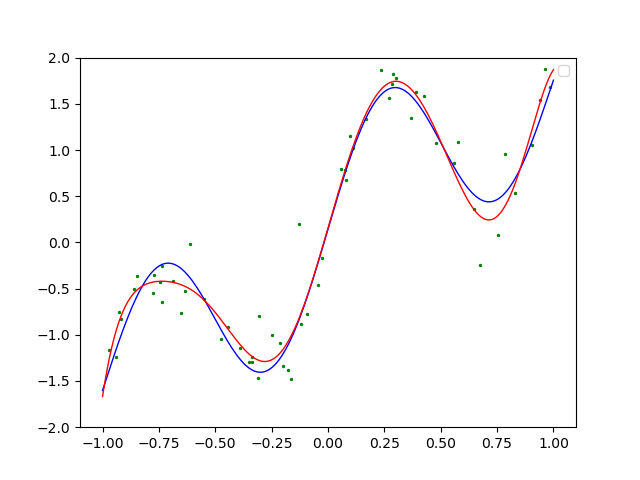
\includegraphics[width=\textwidth]{img/Gaussian_Fit.png}
              \caption{Fitting with 10 Gaussian basis functions. }
              \label{fig:gaussian_basis}
          \end{subfigure}
          \hfill 
          \begin{subfigure}[b]{0.48\textwidth}
          \centering
              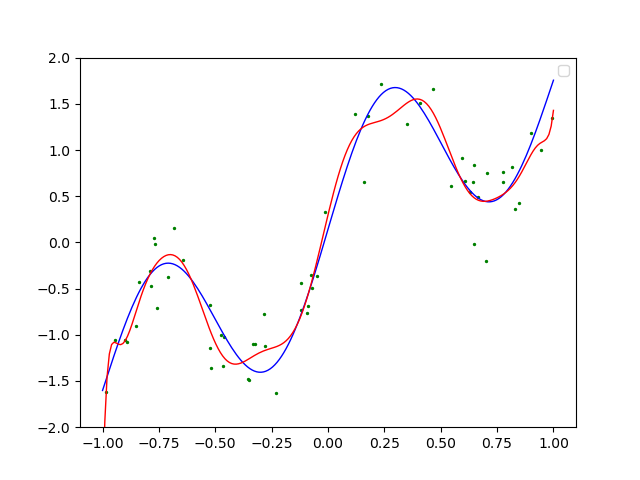
\includegraphics[width=\textwidth]{img/Fourier_Fit.png}
              \caption{Fitting with 10 Fourier basis functions. }
              \label{fig:fourier_basis}
          \end{subfigure}
          \caption{}
          \label{Coincide_mean}
      \end{figure}

    \subsubsection{Standardizing Data}

      \textbf{Standardizing} typically meanss that our featuers will be rescaled to have the properties of a standard normal distribution with mean of $0$ and a standard deviation of $1$. Here are a few methods to scale our data, with their results shown on a dataset of $30$ points in $\mathbb{R}^2$. 
      \begin{enumerate}
          \item \textbf{StandardScaler}: This is probably the most used method for standardizing data. It standardizes features by removing the mean and scaling to unit variance. The standard score of a sample $x^{(n)}$ is $(x - \bar{x})/S$ where $\bar{x}$ is the mean of the training samples and $S$ is the standard deviation of the training samples. 
          \begin{lstlisting}
          from sklearn.preprocessing import StandardScaler
          scaler = StandardScaler()
          scaled_data = scaler.fit_transform(data)
          \end{lstlisting}

          \item \textbf{MinMaxScaler}: While not technically "standardization," MinMaxScaler is another preprocessing method for scaling. It transforms features by scaling each feature to a given range, typically between zero and one, or so that the maximum absolute value of each feature is scaled to unit size. 
          \begin{lstlisting}
          from sklearn.preprocessing import MinMaxScaler
          scaler = MinMaxScaler()
          scaled_data = scaler.fit_transform(data)
          \end{lstlisting}

          \item \textbf{MaxAbsScaler}: This scaler works similarly to the MinMaxScaler but scales in a way that the training data lies within the range $[-1, 1]$ by dividing through the largest maximum value in absolute value. It is meant for data that is already centered at zero or sparse data. 
          \begin{lstlisting}
          from sklearn.preprocessing import MaxAbsScaler
          scaler = MaxAbsScaler()
          scaled_data = scaler.fit_transform(data)
          \end{lstlisting}

          \item \textbf{RobustScaler}: This scaler removes the median and scales the data according to the quantile range (defaults to IQR: Interquartile Range). It's robust to outliers, which makes it a good choice if you have data with possible outliers. 
          \begin{lstlisting}
          from sklearn.preprocessing import RobustScaler
          scaler = RobustScaler()
          scaled_data = scaler.fit_transform(data)
          \end{lstlisting} 

          \item \textbf{QuantileTransformer}: Note that the presence of outliers messes with our scaling. More generally for skewed distributions (like an exponential), a linear transformation does not take care of these outliers, so we would like some nonlinear preprocessing algorithm. One common one is the QuantileTransformer, which takes the quantiles (percentiles) of the dataset and transforms then so that those are equidistant from each other. By default, it divides up the data into 1000 quantiles. 
          \begin{lstlisting}
          from sklearn.preprocessing import QuantileTransformer
          transformer = QuantileTransformer(n_quantiles = 100, output_distribution='normal')
          transformed_data = transformer.fit_transform(data)
          \end{lstlisting}
      \end{enumerate}

      Let's talk about how these scalers will work on some data. We take a wine data with the two variables representing fixed acidity and volatile acidity. 
        \begin{figure}[H]
          \centering
          \begin{subfigure}[b]{0.32\textwidth}
          \centering
              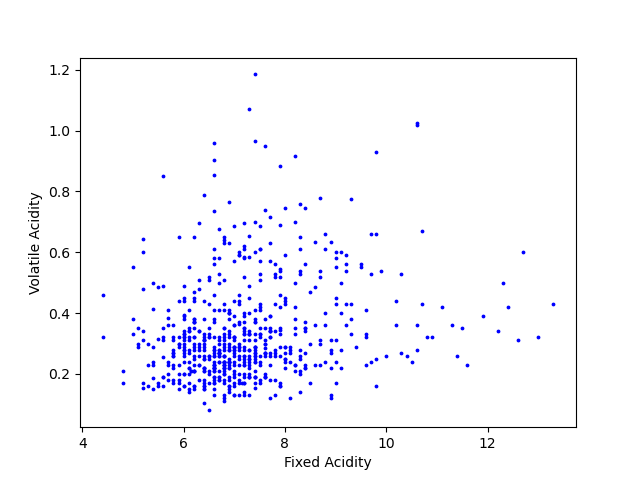
\includegraphics[width=\textwidth]{img/Standard_scaler1.png}
              \caption{Original Data}
              \label{fig:no_scaling}
          \end{subfigure}
          \hfill
          \begin{subfigure}[b]{0.32\textwidth}
          \centering
              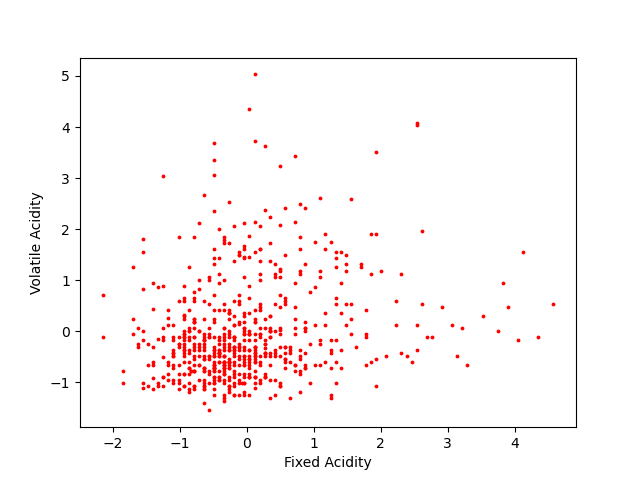
\includegraphics[width=\textwidth]{img/Standard_scaler2.png}
              \caption{StandardScaler}
              \label{fig:standard_scaler}
          \end{subfigure}
          \hfill
          \begin{subfigure}[b]{0.32\textwidth}
          \centering
              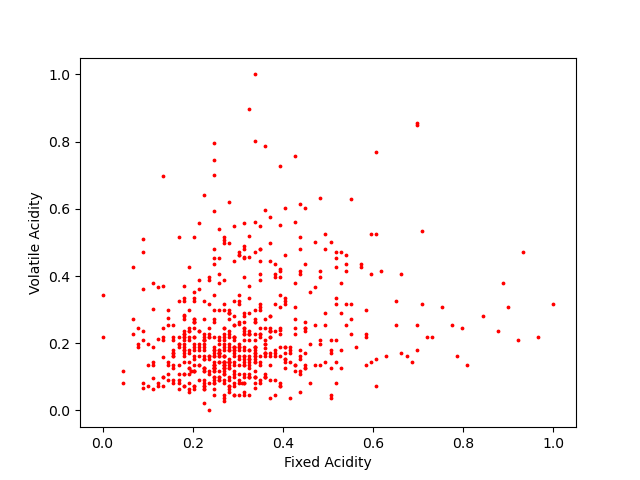
\includegraphics[width=\textwidth]{img/MinMax_Scaler.png}
              \caption{MinMaxScaler}
              \label{fig:minmax_scaler}
          \end{subfigure}

          \begin{subfigure}[b]{0.32\textwidth}
          \centering
              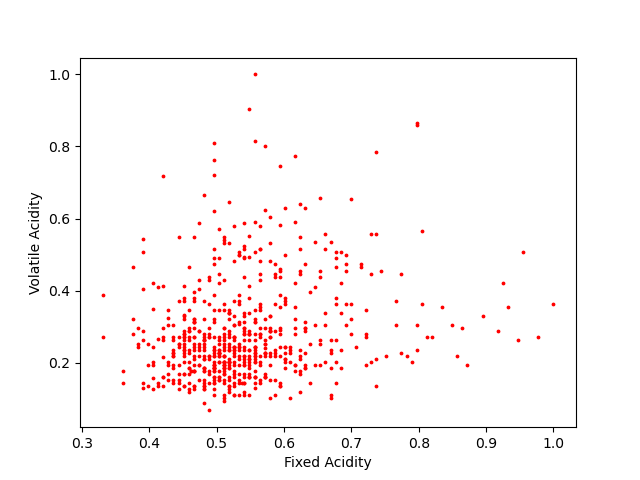
\includegraphics[width=\textwidth]{img/MaxAbs_Scaler.png}
              \caption{MaxAbsScaler}
              \label{fig:maxabs_scaler}
          \end{subfigure}
          \hfill
          \begin{subfigure}[b]{0.32\textwidth}
          \centering
              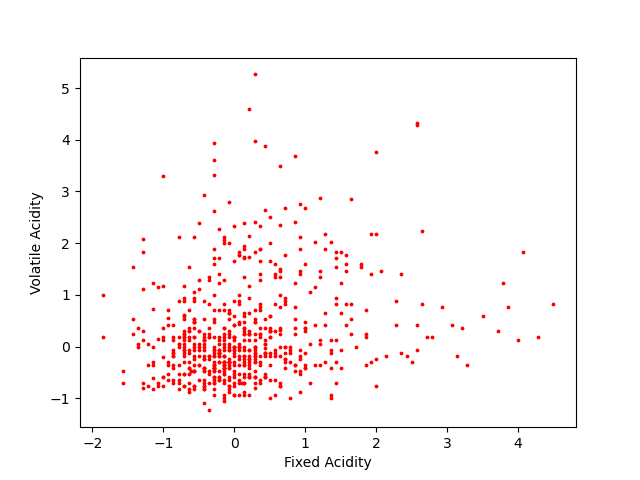
\includegraphics[width=\textwidth]{img/Robust_Scaler.png}
              \caption{RobustScaler}
              \label{fig:robust_scaler}
          \end{subfigure}
          \hfill
          \begin{subfigure}[b]{0.32\textwidth}
          \centering
              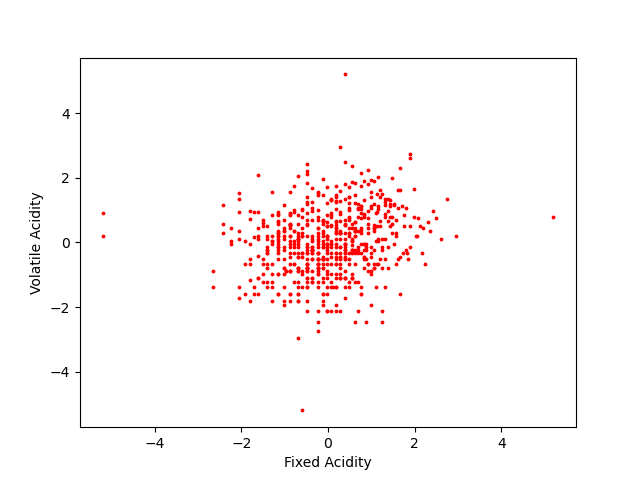
\includegraphics[width=\textwidth]{img/Quantile_Scaler.png}
              \caption{QuantileTransformer}
              \label{fig:quantile_transformer}
          \end{subfigure}
          
          \caption{The StandardScaler simply standardizes the data to have $0$ mean and unit variance.}
          \label{Scalers}
        \end{figure}

      It's important to note that whether you should standardize your data and how you should do it depends on the specific characteristics of your data and the machine learning algorithm you're using. For example, some algorithms, like many in deep learning, assume that all features are on the same scale. Others, like Decision Trees and Random Forests, do not require feature scaling at all. 

  \subsection{Data Augmentation}

